\section{Simulation Tools}

Several simulation tools were used in the development of the CLAS12 Trigger System. These tools were very useful during the development and implementation stages, and are still in use now for continued validation. The primary simulation tools for the CLAS12 Trigger System are detailed below.


\subsection{GEMC/GEANT4 Simulation Tool}

In the beginning of the CLAS12 Trigger System development, the hardware was not available, so input data were generated by the CLAS12 Geant4 Monte-Carlo package (GEMC, \ref{}). This package was used to produce data files with data banks in the same form as produced by the DAQ. The Trigger System software includes a playback package that is able to read GEMC-generated files and produce FADC and DCRB responces identical to the those from the hardware. All Stage 1 trigger components implemented with HLS were developed using simulated data, including for the most complex responces in the calorimeter and drift chambers. For VHDL-written components, simulated data were used as well along with other specialized tools described below.

For example, Fig.~\ref{fig:ecal_sim1} and Fig.~\ref{fig:ecal_sim2} show a comparison of the energy and coordinates of the EC clusters reconstructed by the offline analysis software and by the Trigger System. Different dividing methods were used in the Trigger System, including one based on digital signal processing (DSP) and another based on using lookup tables. The first method provides better results but requires more resources than the second method. Over the course of system development, many decisions were made based on similar comparisons.

\begin{figure}[htp]
	\begin{center}
		\centering
		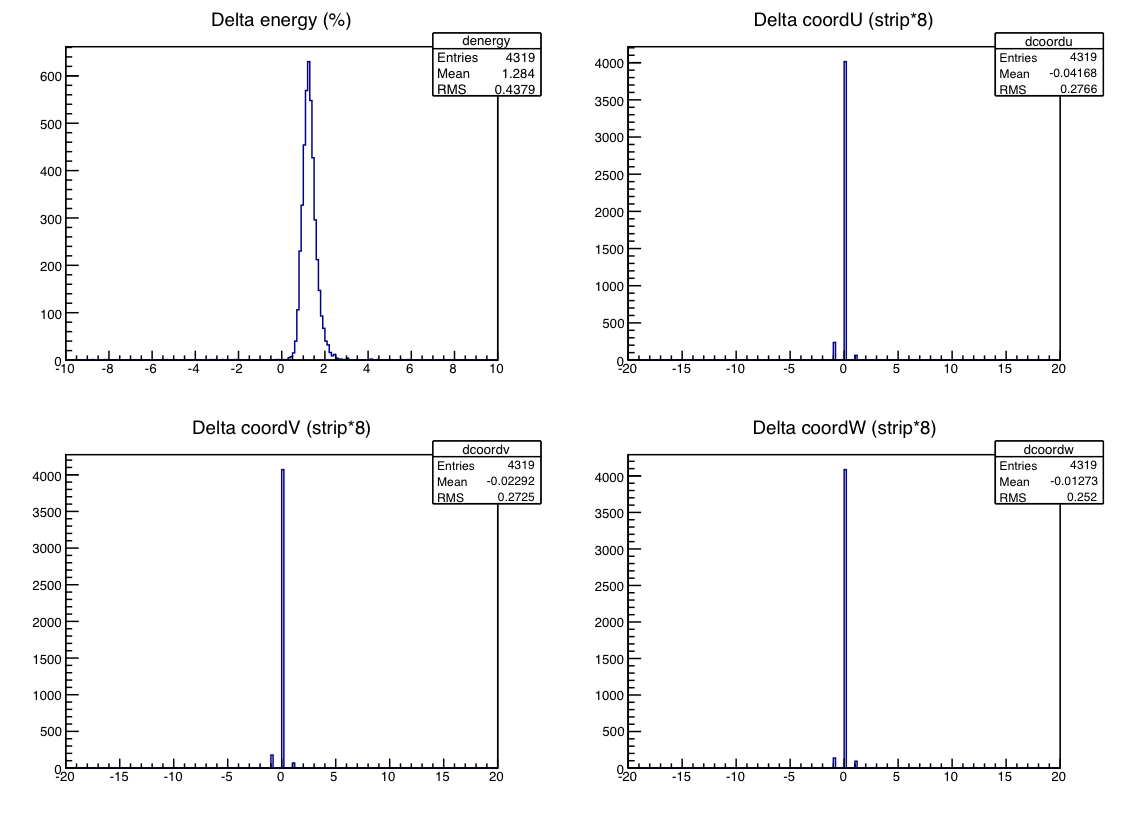
\includegraphics[width=8cm]{img/ecal_sim1.png}
		\caption{EC cluster finding: difference between results from offline reconstruction and trigger system (using dividing in coordinate calculation).}
		\label{fig:ecal_sim1}
	\end{center}
\end{figure} 

\begin{figure}[htp]
	\begin{center}
		\centering
		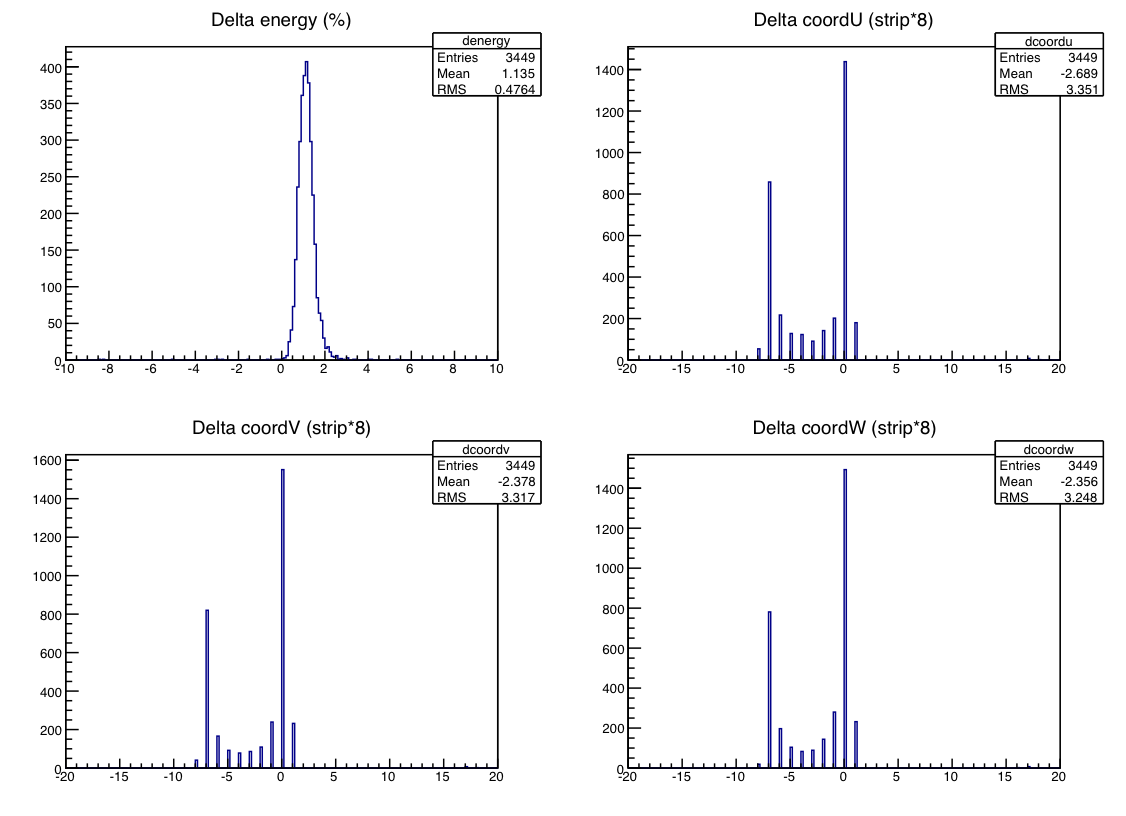
\includegraphics[width=8cm]{img/ecal_sim2.png}
		\caption{EC cluster finding: difference between results from offline reconstruction and trigger system (using lookup table in coordinate calculation).}
		\label{fig:ecal_sim2}
	\end{center}
\end{figure} 

Another example (see Fig.~\ref{fig:ecal_sim3}) shows the absolute EC cluster energy obtained by offline analysis and by the Trigger System. As can be seen, the Trigger System provides the same result as predicted by simulation and obtained from offlne analysis.

\begin{figure}[htp]
	\begin{center}
		\centering
		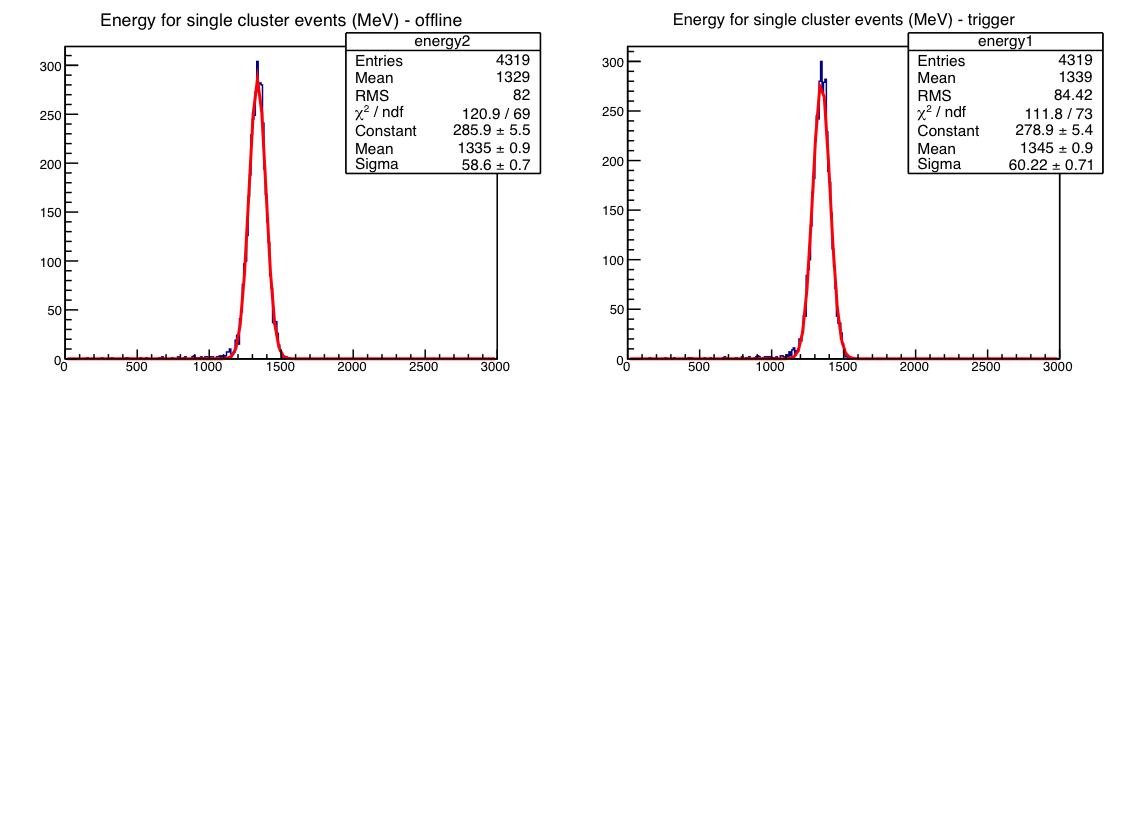
\includegraphics[width=8cm]{img/ecal_sim3.png}
		\caption{EC cluster finding: 5 GeV electron, no PCAL, energy deposition in offline and trigger model.}
		\label{fig:ecal_sim3}
	\end{center}
\end{figure} 


\subsection{FPGA Simulation Tools}

A cycle accurate simulator was setup to model, test, and debug the full Trigger System using Aldec Riviera. This tool is able to perform simulations of the full Trigger System in a mixed language environment (VHDL, Verilog, C/C++) for all FPGA components used in CLAS12 (Xilinx series 5, 6,and 7 components). VHPI was used to interface external C/C++ programs from the DAQ to the VHDL test bench. Using VHPI, calls to the DAQ EVIO (the native DAQ data format) C/C++ libraries were possible from VHDL, making it possible to feed detector waveform data into the trigger simulation directly from Monte Carlo, data files taken with beam, or from user-created text files. Simulation intensive components, primarily gigabit SerDes components, were replaced with fast, simple models once verified to improve the simulation performance. The simulator is single-threaded and requires a license for each running instance, making it costly to parallelize. Even so, it was capable of processing 1 event every 30~s on a typical desktop PC simulating the CLAS12 forward and central Trigger System comprised of 24,192 drift chamber wires and about 3400 FADC channels.

The simulation was built from the actual HDL firmware source files compiled for the various modules used in the trigger system (DCRB, FADC, VTP, SSP). HDL wrappers were created to model the VXS crates which include: backplane, fiber interconnect, trigger distribution, clock distribution, configuration, and readout. The Table~\ref{tab:trig_sim_crates} summarizes the trigger simulation components:

\begin{table}
\begin{center}
	\begin{tabular}{| l | l | l | l | l |}
		\hline \hline
		System		& Crates	& ModType	& ModCnt	& ChCnt		\\
		\hline
		DC			& 18		& DCRB		& 252		& 24192		\\
		ECAL		& 6			& FADC		& 84		& 1296	 	\\
		PCAL		& 6			& FADC		& 96		& 1152	 	\\
		FTOF		& 6			& FADC		& 36		& 576	 	\\
		FTCAL		& 2			& FADC		& 21		& 332	 	\\
		FTHODO		& 1			& FADC		& 15		& 232	 	\\
		CND			& 1			& FADC		& 9			& 144	 	\\
		CTOF		& 1			& FADC		& 6			& 96	 	\\
		HTCC		& 1			& FADC		& 3			& 48	 	\\
		GT			& 1			& SSP		& 6			& 28 (Fiber)	\\
		\hline \hline
	\end{tabular}
\end{center}
\caption{Trigger Simulation crates.}
\label{tab:trig_sim_crates}
\end{table}

Each of the front-end crates uses a VTP trigger module that runs the detector-specific trigger algorithm. The front-end VTP modules feed the trigger data to the global trigger (GT) crate Stage 2 (SSP). The SSP modules feed the trigger data into the final trigger Stage 3 (GTP). There are 10 different VTP firmware types to support the Stage 1 (front-end) and Stage 3 (GTP) algorithm. There are 2 different SSP firmware types that support the Stage 2 CLAS12 Forward and Central Detector trigger logic.

This full simulation is primarily run for two scenarios. The first is whenever a significant firmware change is made. In this case a small number of specially selected events (about 2k) can be fed through to tag the trigger decisions on each. The second is whenever the DAQ system records events where the trigger failed to properly tag them (typically during a random trigger run to assess the efficiency). For both cases the failed events can be loaded into the simulation and the failed decisions can be explored in detail to determine the cause. The first scenario takes one day or more depending on the number of events needed to check, while the second case can take minutes, since only failed events are presented to the simulation so problems can immediately begin to be examined.